\documentclass[a4paper]{article}
\usepackage{amsmath}  % Paquet nécessaire pour \dfrac
\usepackage[utf8]{inputenc}
\usepackage[french]{babel}
\usepackage{graphicx}
\usepackage{array}
\usepackage{fancyhdr}
\usepackage{lastpage} % Paquet pour obtenir le nombre total de pages
\usepackage{geometry} % Paquet pour ajuster les marges
\usepackage[datesep=/,style=ddmmyyyy]{datetime2} % Paquet pour formater la date
\usepackage{setspace} % Inclut le paquet setspace
\usepackage{enumitem}
\usepackage{amssymb} % Pour plus de symboles
\usepackage{indentfirst}
\usepackage{hyperref}
\usepackage{array}
\usepackage{booktabs}

\usepackage{titlesec} % Inclut le paquet titlesec
% Redéfinir le format du titre de la section avec une taille de police plus petite
\titleformat{\section}
{\normalfont\large\bfseries}{\thesection}{1em}{}

% Définition des marges de la page et de l'en-tête
\geometry{
	left=20mm,
	right=20mm,
	top=40mm,
	bottom=30mm,
	headsep=20mm
}

\pagestyle{fancy}
\fancyhf{} % Efface l'en-tête et le pied de page par défaut
\renewcommand{\headrulewidth}{0pt} % Supprime la ligne de l'en-tête
\renewcommand{\footrulewidth}{0.4pt} % Ligne au-dessus du pied de page

\fancyhead[C]{ % Contenu centré dans l'en-tête
	\begin{tabular}{|m{3.5cm}|m{9.0cm}|m{3.5cm}|}
		\hline
		\begin{minipage}[c][2.0cm][c]{3.5cm}
			\centering
			
\includegraphics[width=2.98cm,height=1.25cm]{logo.png}
		\end{minipage} & 
		\begin{minipage}[c][2.0cm][c]{9cm}
			\centering
			\hyphenpenalty=10000 % Évite les césures
			\vspace*{\fill} % Espace vertical flexible avant le texte
			\begin{spacing}{1.5} % Augmente l'espacement entre les lignes à 1,25
				{\large \textbf{Inducteur pour la réduction du courant transitoire \textit{Inrush} dans les condensateurs}}
			\end{spacing}
			\vspace*{\fill} % Espace vertical flexible après le texte
		\end{minipage} & 
		\begin{minipage}[c][2.0cm][c]{3.5cm}
			\raggedleft
			Émission: \DTMtoday \\
			Page: \thepage/\pageref{LastPage}
		\end{minipage} \\
		\hline
	\end{tabular}
}

% Contenu du pied de page
\fancyfoot[L]{%
	\begin{tabular}[b]{@{}l@{}}
		\href{http://www.dax.energy}{www.dax.energy}
	\end{tabular}
}
\fancyfoot[C]{%
	\begin{tabular}[b]{@{}c@{}}
		\href{mailto:comercial@dax.energy}{comercial@dax.energy}
	\end{tabular}
}
\fancyfoot[R]{%
	\begin{tabular}[b]{@{}r@{}}
		+55 41 99940-3744 \\ 3626-2072
	\end{tabular}
}

\begin{document}
	\setstretch{1.25} % Définit l'espacement entre les lignes à 1,25
	
	\section{Contexte}
	L'activation d'une batterie de condensateurs (Figure \ref{fig:picture1}) par la fermeture d'un disjoncteur entraînera un courant de crête transitoire élevé (Figure \ref{fig:picture2}), appelé inrush. L'amplitude et la fréquence de ce courant de crête transitoire dépendent de :
	\begin{itemize}[label=\textendash]
		\item la tension appliquée (point sur l'onde de tension au moment de la fermeture);
		\item la capacitance équivalente du circuit;
		\item l'inductance dans le circuit (quantité et emplacement);
		\item la charge sur la batterie de condensateurs au moment de la fermeture;
		\item tout amortissement du circuit dû à des résistances de fermeture ou à d'autres résistances dans le circuit.
	\end{itemize}
	
	\section{Données d'entrée de la batterie}
	\begin{itemize}[label=\textendash]
		\item Puissance réactive  = {{potencia_reativa_do_banco}}
		\item Tension triphasée  = {{tensao_trifasica}}
		\item Tension monophasée  = {{tensao_monofasica}}
		\item Courant de court-circuit  = {{corrente_de_curto}}
	\end{itemize}
	
	\begin{center}
		% INSERT_TABLE_HERE
	\end{center}
	
	\section{Considérations initiales}
	
	Le courant transitoire \textit{inrush} n'est pas un facteur limitant dans les applications de batteries de condensateurs isolées. Cependant, lorsque les batteries de condensateurs sont commutées en \textit{back-to-back}, c'est-à-dire lorsqu'une batterie est activée alors qu'une autre batterie est connectée au même barreau, des courants transitoires de haute amplitude et de fréquence naturelle élevée circuleront entre la batterie activée et celles qui étaient déjà activées.
	
	\begin{figure}[!hbp]
		\centering
		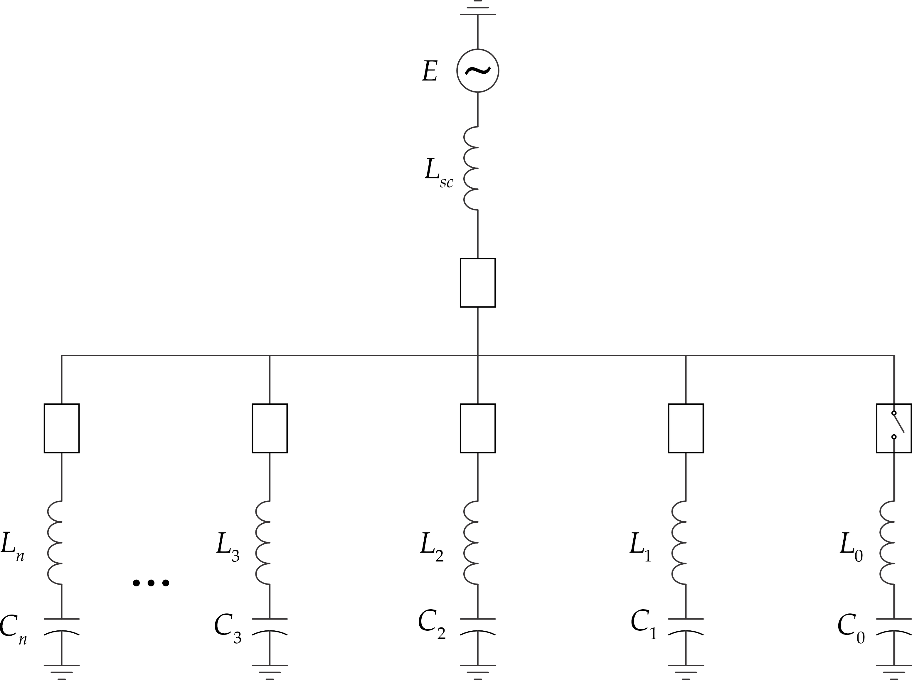
\includegraphics{Picture1.png}
		\caption{Système de batterie de condensateurs.}
		\label{fig:picture1}
	\end{figure}
	
	Ce courant oscillatoire est limité uniquement par l'impédance de la batterie de condensateurs et par le circuit entre la batterie ou les batteries activées et la batterie commutée (Batterie \#0), qui se dissipe généralement en une fraction de cycle de la fréquence du système. Dans le cas d'une commutation \textit{back-to-back}, le composant fourni par la source est à une fréquence plus basse (60 Hz) et tellement faible par rapport au courant \textit{inrush} qu'il peut être négligé \href{https://ieeexplore.ieee.org/document/7035261}{[ANSI/IEEE C37.012-1979]}.
	
	\section{Résultats}
	\begin{figure}[!hbp]
		\centering
		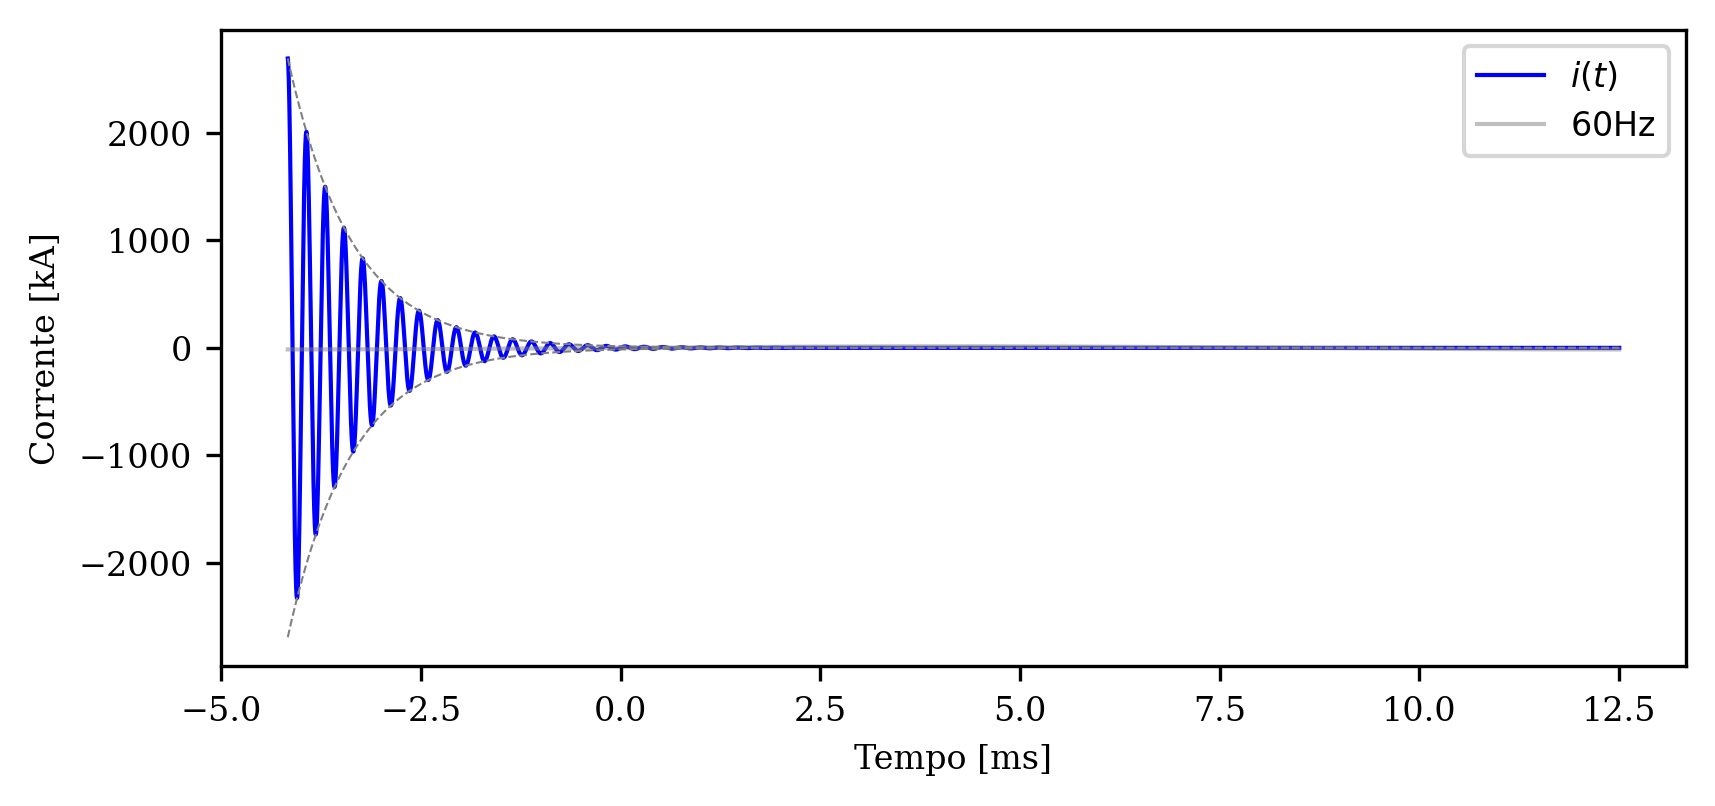
\includegraphics{Correntes.png}
		\caption{Courant instantané dans la batterie de condensateurs activée dans un cycle de la fréquence fondamentale.}
		\label{fig:picture2}
	\end{figure}
	
	Les valeurs obtenues avec le réacteur choisi ($L_{reator} = {{indutancia_escolhida}} \, \mu \rm{H} $) sont :
	\begin{itemize}[label=\textendash]
		\item Courant de crête : {{corrente_pico}};
		\item Fréquence d'oscillation : {{frequencia_oscilacao}}Hz;
		\item Courant inrush / Courant nominal : {{inrush_inominal}}
	\end{itemize}
	
	\section{Conclusion}
	{{conclusao1}}
	
	\section{Références}
	
	\noindent
	\begin{tabular}{p{0.2cm} p{15.8cm}}
		\href{https://ieeexplore.ieee.org/document/7035261}{[1]} &
		\begin{minipage}[t]{15.8cm}
			Guide d'application IEEE pour le commutateur de courant de capacitance pour les disjoncteurs AC haute tension classés sur une base de courant symétrique, dans ANSI/IEEE C37.012-1979, vol., no., pp.1-54, 6 Fév. 1979, doi: 10.1109/IEEESTD.1979.7035261.
		\end{minipage} \\
		
		\href{https://ieeexplore.ieee.org/document/9574631}{[2]} &
		\begin{minipage}[t]{15.8cm}
			Projet de norme approuvé par l'IEEE pour les exigences de commutateurs de condensateurs pour les systèmes AC (1 kV à 38 kV), dans IEEE PC37.66/D10, Octobre 2021, vol., no., pp.1-35, 13 Déc. 2021.
		\end{minipage} \\
		
		
		\href{https://webstore.iec.ch/publication/62785}{[3]} &
		\begin{minipage}[t]{15.8cm}
			Commutateurs et appareillages haute tension IEC 62271-100 - Partie 100: Disjoncteurs à courant alternatif
		\end{minipage} \\
		
		\href{https://ieeexplore.ieee.org/document/5318709}{[4]} &
		\begin{minipage}[t]{15.8cm}
			Norme IEEE pour les disjoncteurs AC haute tension classés sur une base de courant symétrique - Classes préférées et capacités requises pour les tensions supérieures à 1000 V, dans IEEE Std C37.06-2009, vol., no., pp.1-56, 6 Nov. 2009, doi: 10.1109/IEEESTD.2009.5318709.
		\end{minipage} \\
		
		\href{https://cdn.standards.iteh.ai/samples/101972/4e7e06bd66d2443da668b8e0c6c60512/IEC-62271-100-2021.pdf}{[5]} &
		\begin{minipage}[t]{15.8cm}
			Commutateurs et appareillages haute tension IEC 62271-100 - Partie 100: Disjoncteurs à courant alternatif.
		\end{minipage} \\
		
		\href{https://www.normas.com.br/autorizar/visualizacao-nbr/313/identificar/visitante}{[6]} &
		\begin{minipage}[t]{15.8cm}
			NBR 5282 Condensateurs de puissance en dérivation pour système de tension nominale supérieure à 1000 V.
		\end{minipage} \\
	\end{tabular}
	
	% Espace pour les signatures
	\noindent % Empêche l'indentation
	\begin{minipage}[t]{0.5\textwidth} % Commence la première colonne pour la signature
		\centering % Aligne le texte au centre
		\vspace{5cm} % Espace réservé pour la signature
		\rule{6cm}{0.4pt}\\ % Ligne pour signature
		\textbf{Angelo A. Hafner}\\ % Nom
		Ingénieur Électricien\\ % Titre
		CONFEA: 2.500.821.919\\ % Numéro d'enregistrement
		CREA/SC: 045.776-5\\ % Un autre numéro d'enregistrement
		aah@dax.energy % E-mail
	\end{minipage}%
	\hfill % Espace entre les colonnes
	\begin{minipage}[t]{0.5\textwidth} % Commence la deuxième colonne pour la signature
		\centering % Aligne le texte au centre
		\vspace{5cm} % Espace réservé pour la signature
		\rule{6cm}{0.4pt}\\ % Ligne pour signature
		\textbf{Tiago Machado}\\ % Nom
		Directeur Commercial\\ % Titre
		Mobile: +55 41 99940-3744\\ % Contact
		tm@dax.energy % E-mail
	\end{minipage}
	
\end{document}
